\documentclass{article}
\usepackage{pdfpages}
\usepackage{float}
\usepackage{enumerate}
\usepackage{amsmath}
\usepackage{amssymb}
\usepackage{graphicx}
\usepackage{url}
\usepackage{subfig}
\usepackage{color}
\usepackage{hyperref}
\usepackage[margin=0.25in]{geometry}
\hypersetup{
    colorlinks=true,
    linktoc=all
}

\title{3GC3 Final Project}
\author{Emily Horsman}
\date{December 2018}

\begin{document}

\maketitle

\begin{figure}[H]
    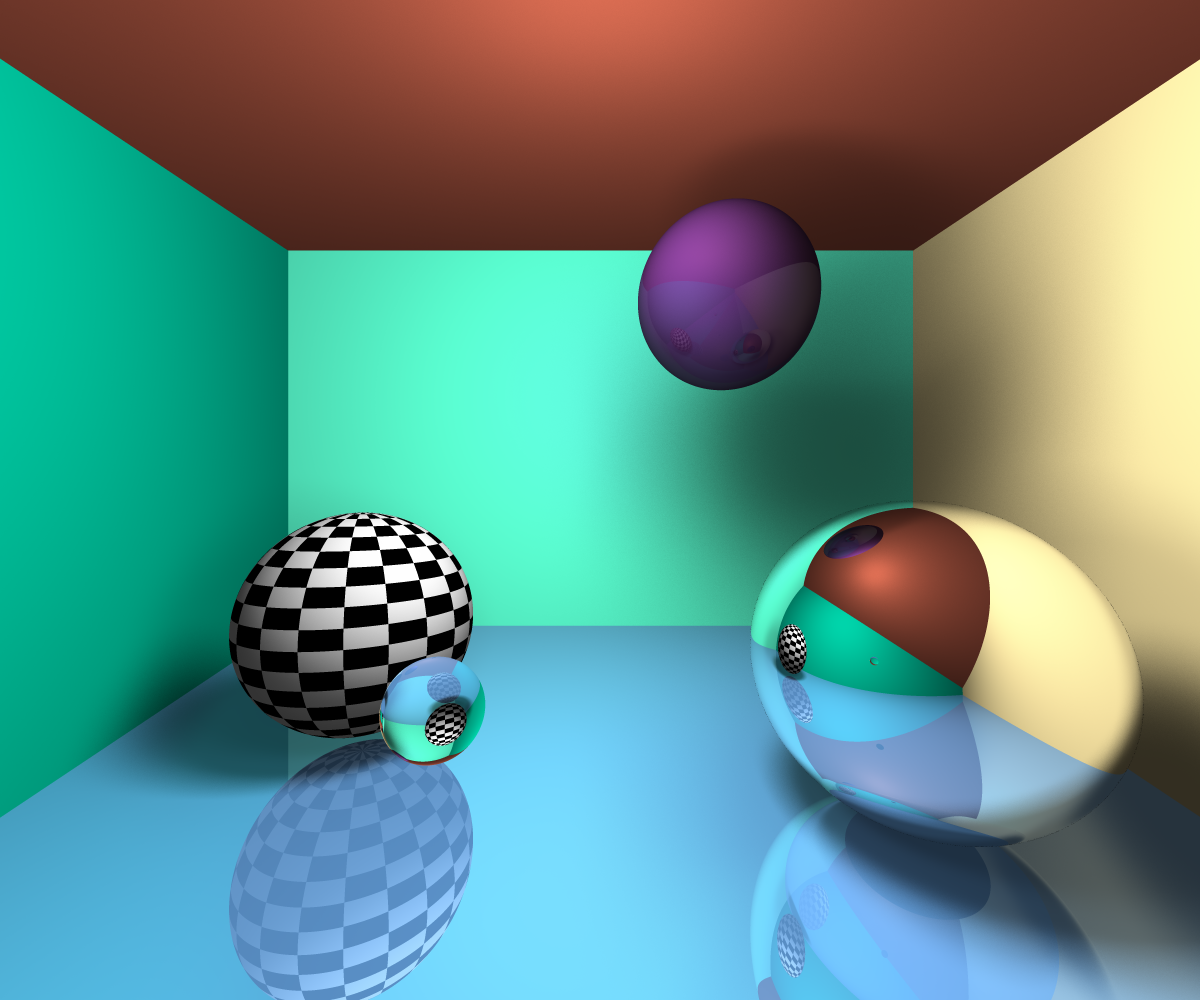
\includegraphics[width=\textwidth]{./examples/SphereRoom.png}
    \caption{Reflective floor, 100\% transparent sphere showing refraction, checkered sphere with texture mapping, mirror sphere. 64x random sampled anti-aliasing with 300 iterations for soft shadows. 13h50m of CPU time.}
\end{figure}

\newpage
\tableofcontents

\section{Feature Overview}

\begin{itemize}
    \item CPU-based ray tracer
    \item Output to PPM bitmaps and a GLUT window
    \item Scene files for configuring rendering and scene parameters, materials, lights, and objects
    \item Support for planes, spheres, and disks
    \item Color and checkered material with proper texture mapping for spheres
    \item Materials specify coefficients for: ambient, diffuse, and specular light; transmission; index of refraction
    \item Multi-threaded rendering with a configurable number of threads
    \item Rudimentary refraction (no Fresnel effect)
    \item Soft shadows achieved by ``jittering'' point lights and averaging multiple renders
    \item Anti-aliasing with both regular (uniform) and random sampling techniques
    \item Adjustable depth-of field and camera field of view
\end{itemize}

\section{Scene Files}

\section{Depth of Field}

\begin{figure}[H]
    \centering
    \subfloat[\texttt{DepthOfField.scene}]{{ 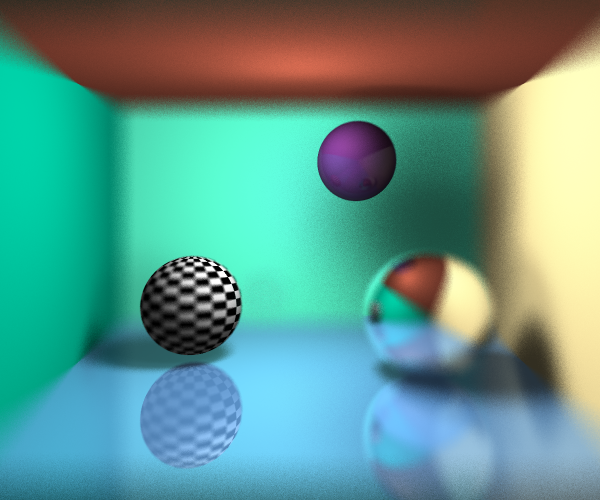
\includegraphics[width=0.45\textwidth]{./examples/DepthOfField.png} }}
    \subfloat[\texttt{DepthOfField2.scene}]{{ 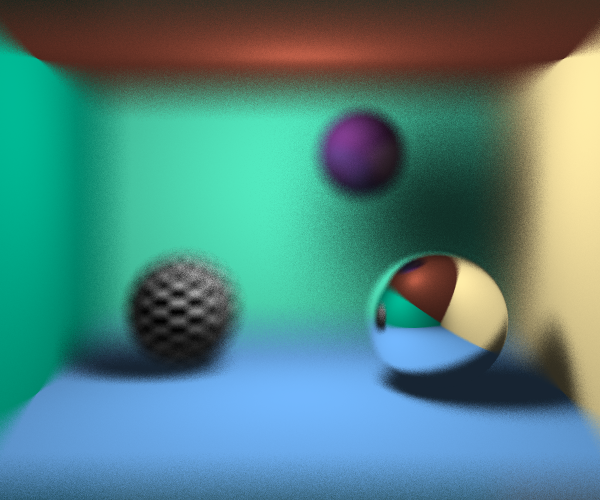
\includegraphics[width=0.45\textwidth]{./examples/DepthOfField2.png} }}
    \caption{A scene displayed with two different focal points. Minimal noise reduction, could be increased.}
\end{figure}

\section{Soft Shadows}

TODO

\section{Refraction}

\begin{figure}[H]
    \centering
    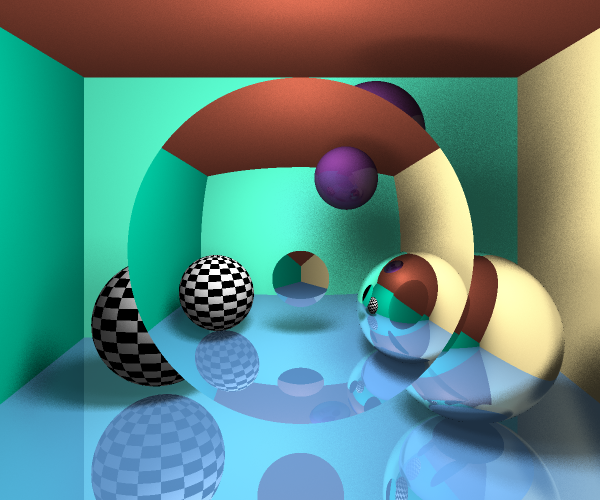
\includegraphics[width=0.6\textwidth]{./examples/DiskLens.png}
    \caption{\texttt{DiskLens.scene}. A 100\% transparent disk with a refractive index of 2.5 placed in front of the scene.}
\end{figure}

\section{Reflection}

\begin{figure}[H]
    \centering
    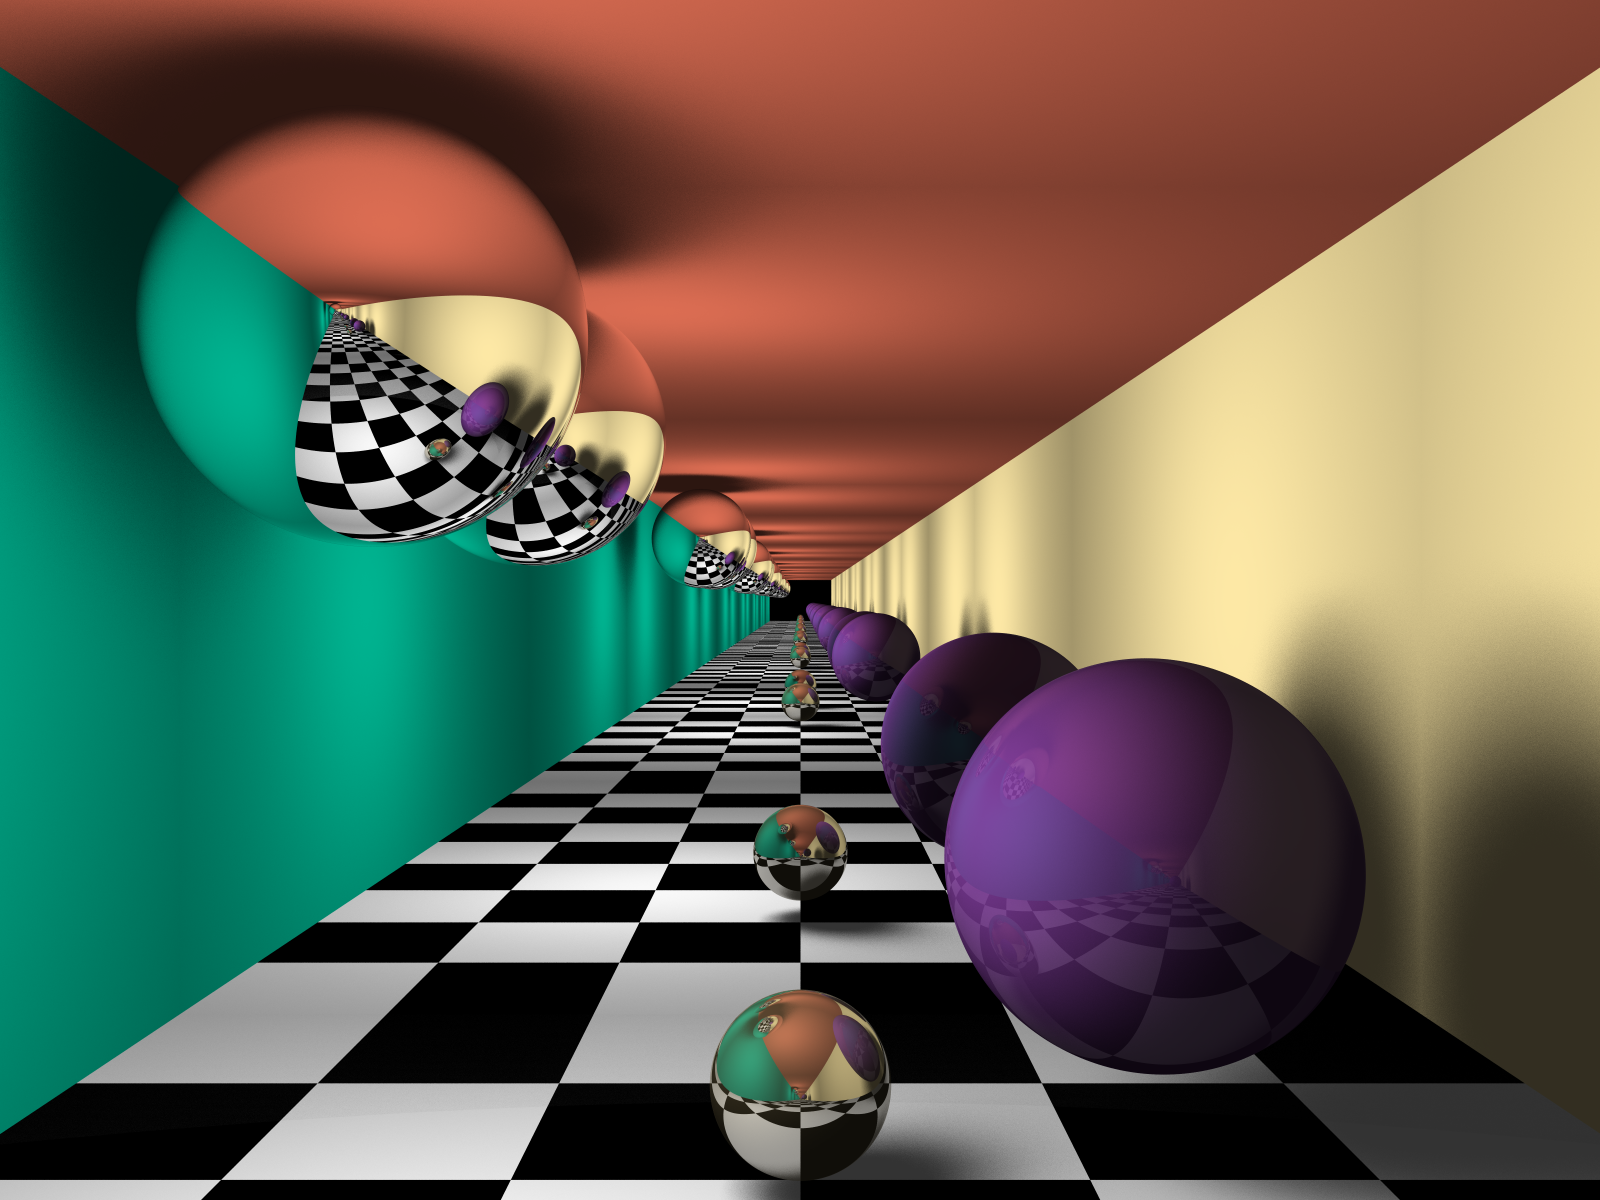
\includegraphics[width=0.6\textwidth]{./examples/HallOfMirrors.png}
    \caption{\texttt{HallOfMirros.scene}. Hall of mirrors with a maxDepth of 15.}
\end{figure}

\begin{figure}[H]
    \centering
    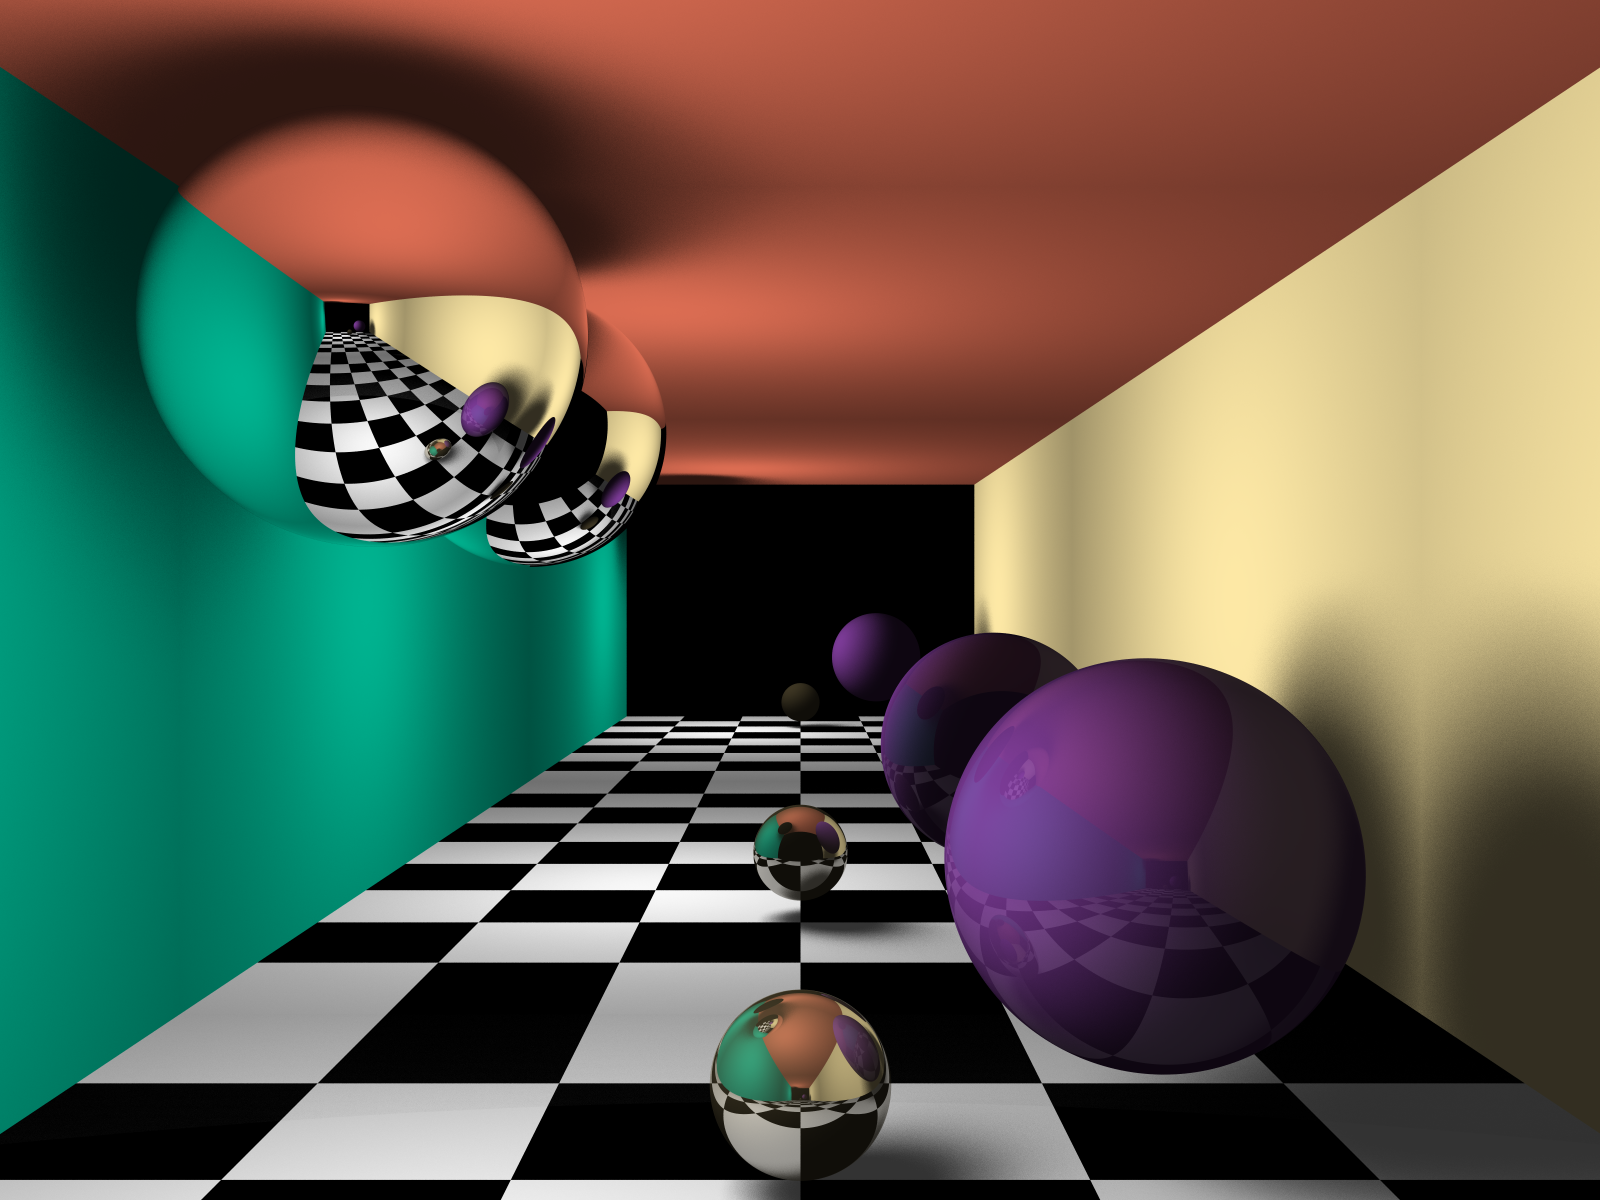
\includegraphics[width=0.6\textwidth]{./examples/HallOfMirrorsDepth2.png}
    \caption{\texttt{HallOfMirros.scene}. Hall of mirrors with a maxDepth of 2.}
\end{figure}

\begin{figure}[H]
    \centering
    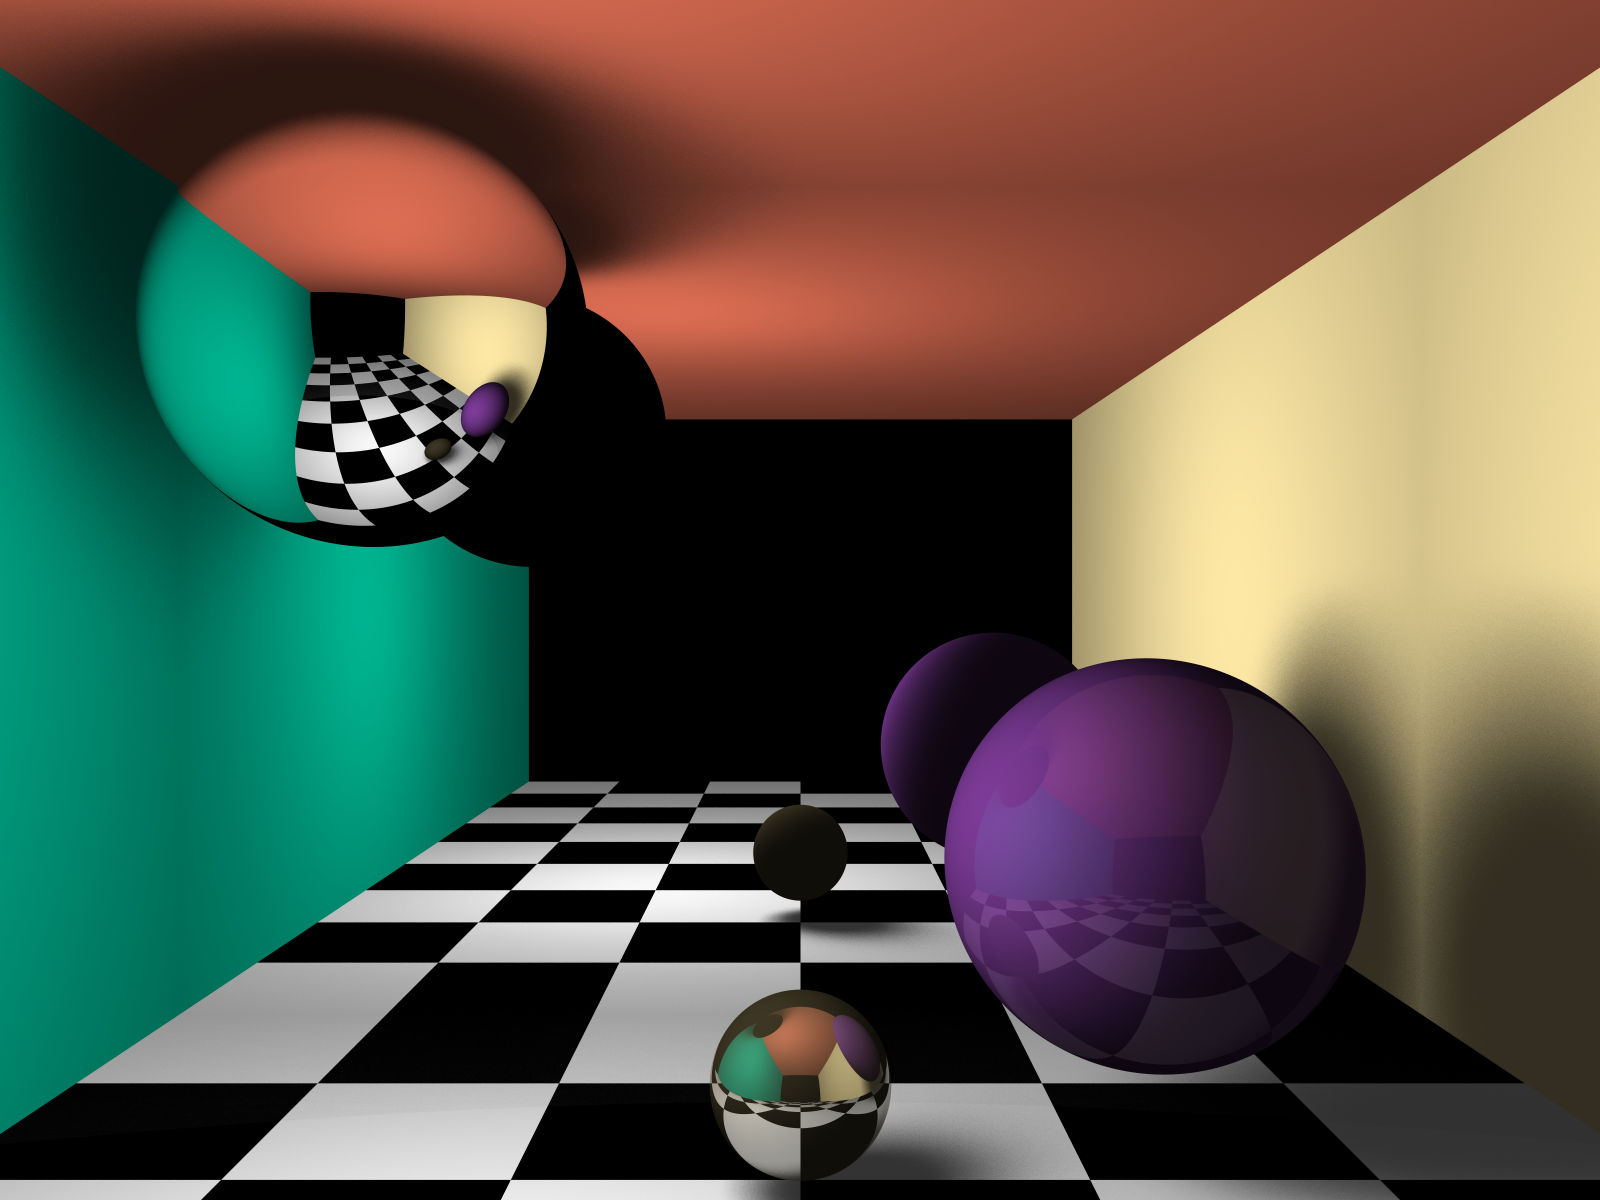
\includegraphics[width=0.6\textwidth]{./examples/HallOfMirrorsDepth3.png}
    \caption{\texttt{HallOfMirros.scene}. Hall of mirrors with a maxDepth of 1.}
\end{figure}

\section{Objects}

\subsection{Types}

TODO

\subsection{Texture}

TODO

\section{Anti-Aliasing}

\begin{figure}[H]
    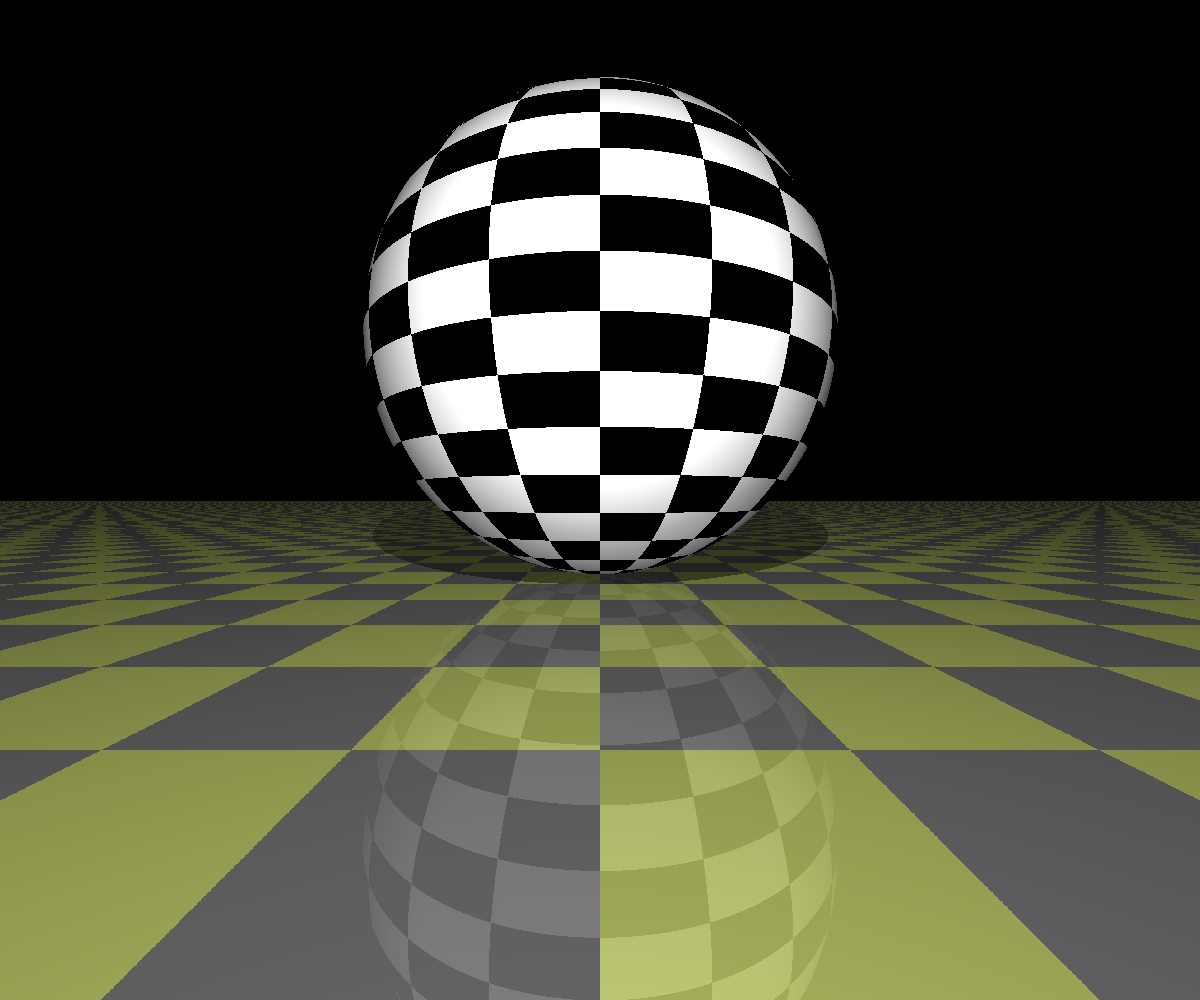
\includegraphics[width=\textwidth]{./examples/AntiAliasingComparison/Scene_noAntiAliasing.png}
    \caption{No anti-aliasing.}
\end{figure}

\begin{figure}[H]
    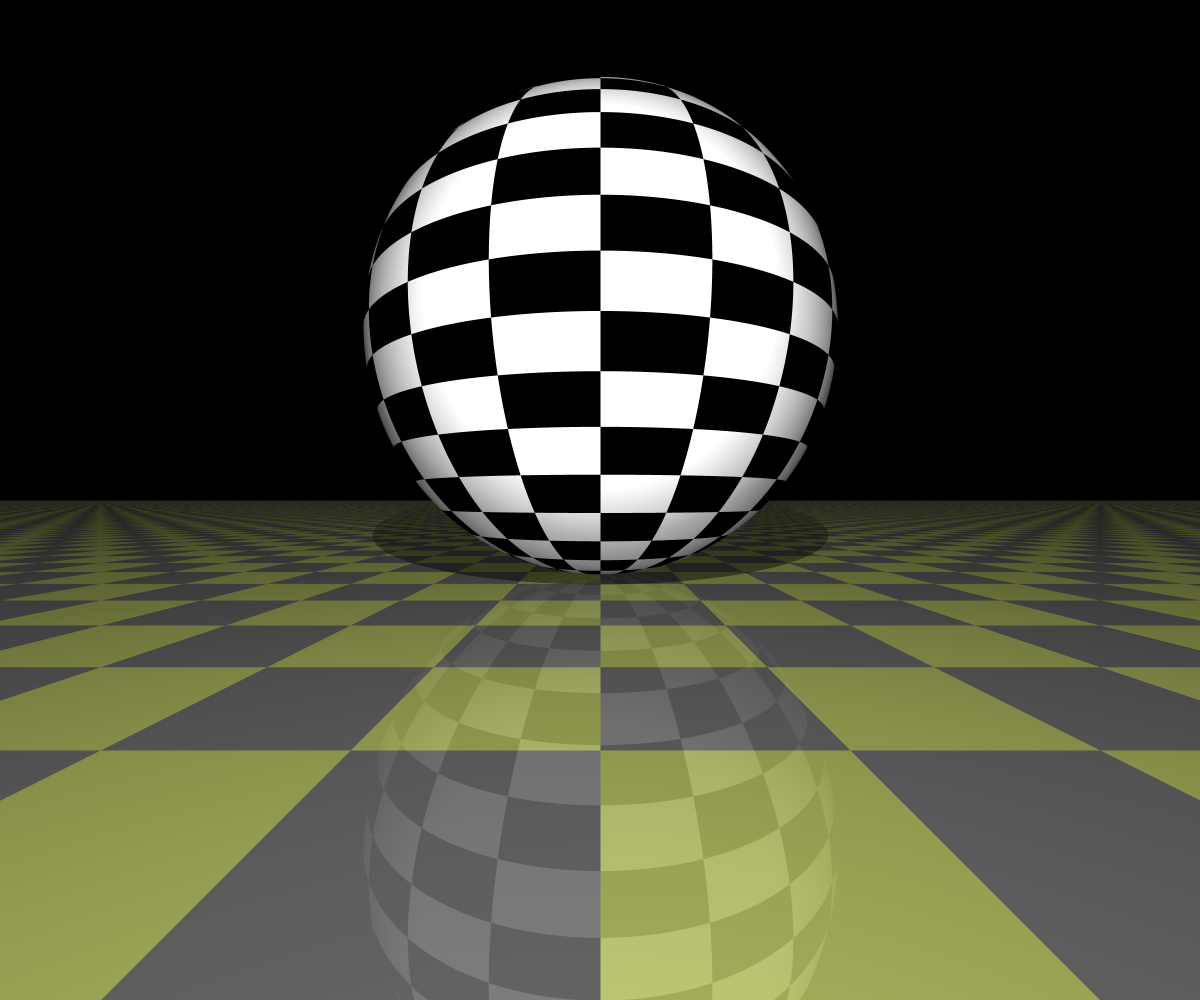
\includegraphics[width=\textwidth]{./examples/AntiAliasingComparison/Scene_regular64.png}
    \caption{64x AA using regular sampling.}
\end{figure}

\begin{figure}[H]
    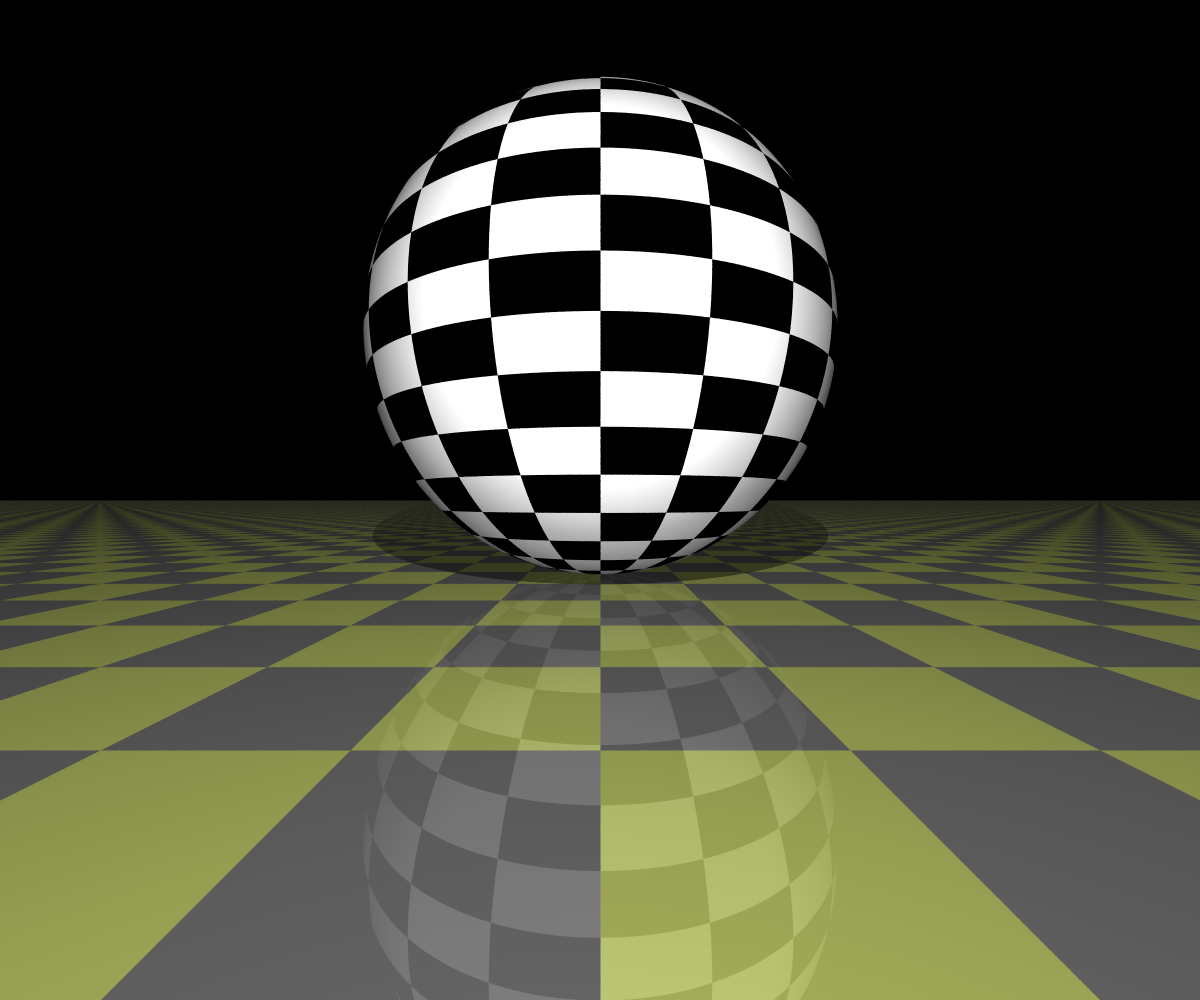
\includegraphics[width=\textwidth]{./examples/AntiAliasingComparison/Scene_random64.png}
    \caption{64x AA using random sampling.}
\end{figure}

\pagebreak

\begin{figure}[H]
    \centering
    \subfloat[Plane]{{ 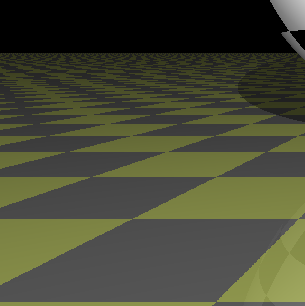
\includegraphics[width=0.3\textwidth]{./examples/AntiAliasingComparison/CheckeredPlane_noAntiAliasing.png} }}
    \subfloat[Sphere]{{ 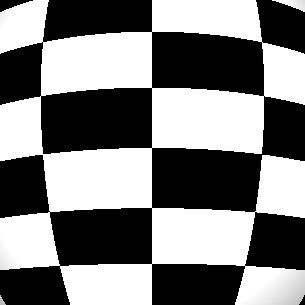
\includegraphics[width=0.3\textwidth]{./examples/AntiAliasingComparison/CheckeredSphereCrop_noAntiAliasing.png} }}
    \caption{Vanishing plane and checkered sphere without anti-aliasing.}
\end{figure}

\begin{figure}[H]
    \centering
    \subfloat[Plane]{{ 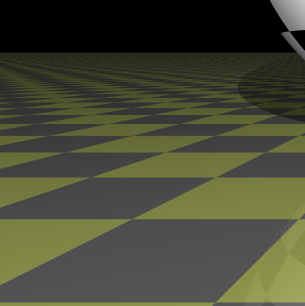
\includegraphics[width=0.3\textwidth]{./examples/AntiAliasingComparison/CheckeredPlane_regular64.png} }}
    \subfloat[Sphere]{{ 
\includegraphics[width=0.3\textwidth]{./examples/AntiAliasingComparison/CheckeredSphereCrop_regular64.png} }}
    \caption{Vanishing plane and checkered sphere with 64x AA using regular sampling.}
\end{figure}

\begin{figure}[H]
    \centering
    \subfloat[Plane]{{ 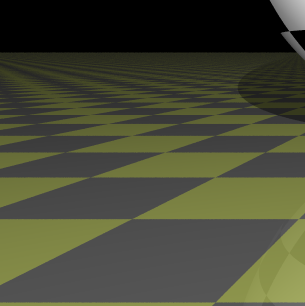
\includegraphics[width=0.3\textwidth]{./examples/AntiAliasingComparison/CheckeredPlane_random64.png} }}
    \subfloat[Sphere]{{ 
\includegraphics[width=0.3\textwidth]{./examples/AntiAliasingComparison/CheckeredSphereCrop_random64.png} }}
    \caption{Vanishing plane and checkered sphere with 64x AA using random sampling.}
\end{figure}

\section{References}

These items are referred to throughout the codebase with \texttt{[n]}.

\begin{enumerate}
    \item https://www.scratchapixel.com/lessons/3d-basic-rendering/ray-tracing-generating-camera-rays/generating-camera-rays
    \item http://www.3dkingdoms.com/weekly/weekly.php?a=2
    \item https://www.scratchapixel.com/lessons/3d-basic-rendering/introduction-to-shading/reflection-refraction-fresnel
    \item https://graphics.stanford.edu/courses/cs148-10-summer/docs/2006--degreve--reflection\_refraction.pdf
    \item Chapter 10 of ``Ray Tracing from the Ground Up'' (Kevin Suffern)
    \item http://cg.skeelogy.com/depth-of-field-using-raytracing/
    \item https://stackoverflow.com/a/13686064/4909532
    \item https://www.scratchapixel.com/lessons/3d-basic-rendering/minimal-ray-tracer-rendering-simple-shapes/ray-sphere-intersection
    \item https://people.cs.clemson.edu/~dhouse/courses/405/notes/texture-maps.pdf
    \item Exercise 18.1 from ``Ray Tracing from the Ground Up'' (Kevin Suffern) p.350
\end{enumerate}

\end{document}
